%% LyX 2.2.2 created this file.  For more info, see http://www.lyx.org/.
%% Do not edit unless you really know what you are doing.
\RequirePackage{fix-cm}
\RequirePackage{fixltx2e}
\documentclass[english]{elsarticle}
\usepackage[T1]{fontenc}
\usepackage{float}
\usepackage{units}
\usepackage{amsmath}
\usepackage{graphicx}
\usepackage{esint}
\usepackage{nomencl}
% the following is useful when we have the old nomencl.sty package
\providecommand{\printnomenclature}{\printglossary}
\providecommand{\makenomenclature}{\makeglossary}
\makenomenclature

\makeatletter

%%%%%%%%%%%%%%%%%%%%%%%%%%%%%% LyX specific LaTeX commands.
%% Because html converters don't know tabularnewline
\providecommand{\tabularnewline}{\\}

%%%%%%%%%%%%%%%%%%%%%%%%%%%%%% Textclass specific LaTeX commands.
\numberwithin{figure}{section}
\numberwithin{equation}{section}
\numberwithin{table}{section}

%%%%%%%%%%%%%%%%%%%%%%%%%%%%%% User specified LaTeX commands.
% specify here the journal
\journal{Example: Nuclear Physics B}

% use this if you need line numbers
%\usepackage{lineno}

\@ifundefined{showcaptionsetup}{}{%
 \PassOptionsToPackage{caption=false}{subfig}}
\usepackage{subfig}
\makeatother
\usepackage{amsopn}
\DeclareMathOperator{\erf}{erf}



\usepackage{geometry}
%\usepackage{babel}
\usepackage{gensymb}


\usepackage[T1]{fontenc}   
\usepackage{bigfoot}% to allow verbatim in footnote
\usepackage[numbered,framed]{matlab-prettifier}
\numberwithin{equation}{subsection}
\usepackage{babel}
\begin{document}
\begin{frontmatter}

\title{MAE 820 Project 2}

\author{D. W. Gould}

\end{frontmatter}\pagebreak{}\newgeometry{left=4cm,right=4cm,top=2cm,bottom=2.5cm}\tableofcontents{}

\pagebreak{}\printnomenclature[2cm]{}

\pagebreak{}

\section{Introduction}

In this project, the finite difference method was used to solve the
lid driven cavity problem. The effectiveness of each solver used was
also analyzed and additional suggestions for further reductions in
computational times were presented.\nomenclature[zomegaopt]{$\omega_{opt}$}{Relaxation parameter - optimal value}\nomenclature[zomega]{$\omega$}{Relaxation parameter}\nomenclature[zpsi]{$\psi$}{Stream function}\nomenclature[zbeta]{$\beta$}{$\nicefrac{\Delta x}{\Delta y}$}\nomenclature[i]{i}{Spatial index, x-dir}\nomenclature[j]{j}{Spatial index, y-dir}\nomenclature[k]{k}{Iteration index}

\section{Model}

\subsection{Geometry}

\begin{figure}
\centering\includegraphics[width=0.5\textwidth]{../../../Desktop/Project1/Diagram3}\caption{Diagram of model geometry \label{fig:Diagram}}
\end{figure}
In Figure \ref{fig:Diagram}, a basic diagram of the geometry is shown.

\subsection{Governing Equations\label{subsec:Governing-Equations}}

Com, ComxComy

\subsection{Discretization and Boundary Conditions}

The governing equations of Section \ref{subsec:Governing-Equations}
were discretized using a staggered grid. Figure \ref{fig:Grid}shows
the node staggering method used in this work for an example grid consisting
of 25 interior pressure nodes.

\begin{equation}
\frac{\partial^{2}\psi}{\partial x^{2}}+\frac{\partial^{2}\psi}{\partial y^{2}}=0\label{eq:Stream}
\end{equation}

Aproximating each of the second derivatives in Equation \ref{eq:Stream}
with second order central differencing scheme results in the discretized
Equation \ref{eq:Discret}. In this work a uniform grid with $\Delta x$
= $\Delta y$ = 0.25m was used. For boundary conditions, all exterior
nodes - with the exception of those located between the points A and
B - were defined to have a constant value of $\psi$=1. The nodes
located at and between points A and B were defined to have a constant
value of $\psi$=0. The mesh used in this work can be seen in Figures
\ref{fig:Part1Solution}, \ref{fig:Re1Results}, \ref{fig:Mod}, and
\ref{fig:Barrier}.

\begin{equation}
\frac{\psi_{i+1,j}-2\psi_{i,j}+\psi_{i-1,j}}{\left(\Delta x\right)^{2}}+\frac{\psi_{i,j+1}-2\psi_{i,j}+\psi_{i,j-1}}{\left(\Delta y\right)^{2}}=0\label{eq:Discret}
\end{equation}

\begin{figure}

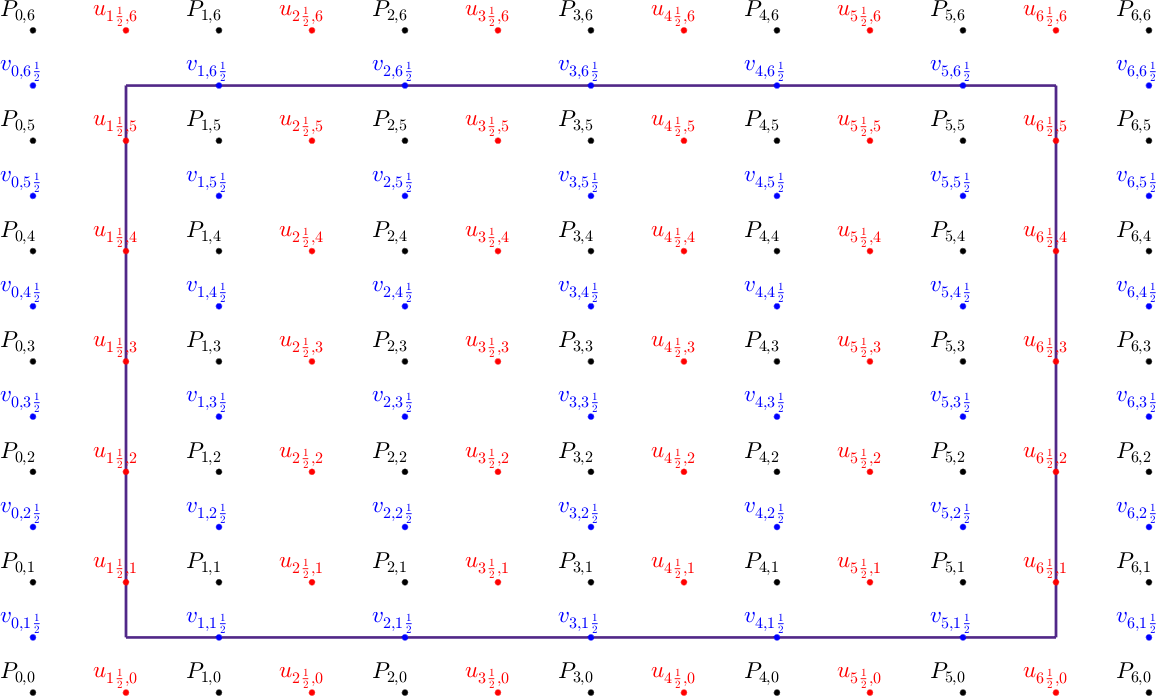
\includegraphics[width=0.5\textwidth]{SixPointGrid}\caption{Example of staggered grid \label{fig:Grid}}

\end{figure}


\section{Solution Method}

\subsection{Projection Method}

In this work, Equation \ref{eq:Discret} was solved using several
different iterative methods. Three of the methods used were explicit
methods. The formula for each of these methods are provided as Equations
\ref{eq:Jacobi} - \ref{eq:SOR}.

In each of these three equations, the variable $k$ indicates the
level of iteration. The simplest of the three methods - that is, the
Jacobi method shown in Equation \ref{eq:Jacobi} - calculates the
new value of stream at the point of interest simply as a function
of the values of the of the surrounding nodes in the previous iteration
step.

The Gauss-Seidel (GS) algorithm, shown in Equation \ref{eq:GS}, improves
on the efficiency of the Jacobi algorithm by incorporating the most
recent values obtained for its adjacent nodes in its calculations.
Thus, while the GS algorithm will not provide any per-iteration reductions
computational time, its use of adjacent node values from the current
iteration level where available should allow it to converge more quickly
than the baseline Jacobi method.

\[
\beta=\frac{\Delta x}{\Delta y}
\]

\begin{equation}
\psi_{i,j}^{k+1}=\frac{\psi_{i+1,j}^{k}+\psi_{i-1,j}^{k}+\beta^{2}\left(\psi_{i,j+1}^{k}+\psi_{i,j-1}^{k}\right)}{2\left(1+\beta^{2}\right)}\label{eq:Jacobi}
\end{equation}

\begin{equation}
\psi_{i,j}^{k+1}=\frac{\psi_{i+1,j}^{k}+\psi_{i-1,j}^{k+1}+\beta^{2}\left(\psi_{i,j+1}^{k}+\psi_{i,j-1}^{k+1}\right)}{2\left(1+\beta^{2}\right)}\label{eq:GS}
\end{equation}

\begin{equation}
\psi_{i,j}^{k+1}=\left(1-\omega\right)\psi_{i,j}^{k}+\omega\frac{\psi_{i+1,j}^{k}+\psi_{i-1,j}^{k+1}+\beta^{2}\left(\psi_{i,j+1}^{k}+\psi_{i,j-1}^{k+1}\right)}{2\left(1+\beta^{2}\right)}\label{eq:SOR}
\end{equation}

Equation \ref{eq:SOR} shows the general formula for the Successive
Over-Relaxation (SOR) method. The SOR method improves on the GS solution
method by incorporating over - or, if increased stability is desired,
under - relaxation into the equation using the relaxation parameter
$\omega$. When $\omega$ is equal to 1, the SOR method becomes identical
to the GS method. Raising $\omega$ to values greater than one can
increase the rate of convergence at the cost of stability. Conversely,
lowering the relaxation parameter below unity will result in dramatically
increased computational times, but provides greater stability.

\subsection{Poisson Solver}

Two different partially implicit solution methods were used, Successive
Over-Relaxation by Lines (SLOR) and the Alternating Direction Implicit
(ADI) method. In Equation \ref{eq:SLOR}, three unknown values are
present. These unknowns are the value of the stream function at the
central point, $\psi_{i,j}^{k+1}$, and the values at the the two
points adjacent to the central point on row $j$.\textless{}\textless{}\textless{}\textless{}\textless{}\textless{}\textless{}
HEAD:Project22.lyx Interpolation was used whenever the scheme required
information at a location between nodes.

Examples of this discretization for some of the terms in Equations
\ref{eq:DiscTime} \textendash{} \ref{eq:N+1} are given in Equations
\ref{eq:DiscEx1} and \ref{eq:DiscEx2}.

\begin{equation}
\left[\frac{\partial}{\partial x}\left(u^{2}\right)\right]_{i+\frac{1}{2},j}=\frac{\left(u_{i+1,j}\right)^{2}-\left(u_{i,j}\right)^{2}}{\Delta x}\label{eq:DiscEx1}
\end{equation}

\begin{equation}
\left[\frac{\partial}{\partial y}\left(uv\right)\right]_{i+\frac{1}{2},j}=\frac{\left(uv\right)_{i+\frac{1}{2},j+\frac{1}{2}}-\left(uv\right)_{i+\frac{1}{2},j-\frac{1}{2}}}{\Delta y}\label{eq:DiscEx2}
\end{equation}

For the $u$ ======= Solving this equation requires that an implicit method be used so that the values of 
 can be solved for the entire row $j$ simultaneously.

While more difficult to implement, this method has the major advantage
that it communicates information from the BC at the ends of each row
instantly in a single iteration. This is in contrast to the very slow
dispersal of information found in the aforementioned explicit methods
in which it could take 7 iterations for a node in the center of the
domain might to be affected by a change in the boundary conditions.

For the ADI method, the principal remains the same. However, instead
of each iteration consisting of solving the domain row by row, in
the Alternating Direction Implicit method will follow a sweep of the
rows of a domain with a similar sweep of the columns of a domain.
This method allows information from each extremity of the domain to
quickly propagate to the center. The equation used for the ADI method
is the same as that used for the SLOR method, but which terms are
known and which terms are solved for depend on the direction of the
sweep.

\begin{equation}
\psi_{i,j}^{k+1}=\left(1-\omega\right)\psi_{i,j}^{k}+\frac{\omega}{2\left(1+\beta^{2}\right)}\psi_{i+1,j}^{k+1}+\psi_{i-1,j}^{k+1}+\beta^{2}\left(\psi_{i,j+1}^{k}+\psi_{i,j-1}^{k+1}\right)\label{eq:SLOR}
\end{equation}


\subsubsection{Thomas Algorithm}

The tridiagonal matrices resulting from the implementation of both
the SLOR and ADI methods was simultaneously solved using the Thomas
Algorithm. While only valid for sparse, tridiagonal matrices such
as those created by the SLOR and ADI methods, the Thomas Algorithm
can theoretically be made to be highly efficient. The general algorithm
consists of working down each row of the matrix, eliminating the subdiagonal
term in each row. This results in an upper diagonalizing of the equation
matrix, allowing for the unknown stream values to be obtained by back
substitution. The specific code written to do this can be found in
Appendix \ref{subsec:Thomas-Algorithm}.

\section{Results - Part 1}

The inital conditons used and results obtained for part one can be
seen in Figure \ref{fig:Part1Solution}. In each of these figures,
the mesh used is overlayed.

\begin{figure}[h]
\centering%
\begin{minipage}[c]{0.49\textwidth}%
\subfloat[Part 1 initial conditions with mesh overlay\label{fig:Part1IC}]{\centering\includegraphics[clip,width=1\linewidth]{../../../Desktop/Project1/IC1}

}%
\end{minipage}\hfill{}\centering%
\begin{minipage}[c]{0.49\textwidth}%
\subfloat[Part one solution with mesh overlay \label{fig:Part1Psedo}]{\bigskip{}
\centering\includegraphics[clip,width=1\linewidth]{../../../Desktop/Project1/Solution1}

}%
\end{minipage}\caption{Solution of part 1 \label{fig:Part1Solution}}
\end{figure}

In Figure \ref{fig:ErrorPlots}, the effects each solver on the convergence
of the solution is shown. A convergence criteria of 1E-8 was used
solvers in this project.

\begin{figure}[h]
\centering%
\begin{minipage}[c]{0.49\textwidth}%
\subfloat[Error vs iteration number for each solver\label{fig:Norm2Error}]{\centering\includegraphics[clip,width=1\linewidth]{../../../Desktop/Project1/ErrorCompare1}

}%
\end{minipage}\hfill{}\centering%
\begin{minipage}[c]{0.49\textwidth}%
\subfloat[Comparison of norm 1, norm 2, norm$\infty$ error\label{fig:ErrorCompare}]{\centering\includegraphics[clip,width=1\linewidth]{../../../Desktop/Project1/NormCompare1}

}%
\end{minipage}\caption{Relative error from examined solution methods \label{fig:ErrorPlots}}
\end{figure}

\begin{table}
\centering

\begin{tabular}{|c|c|c|c|c|c|}
\hline 
 & \textbf{Jacobi} & \textbf{G-S} & \textbf{SOR} & \textbf{SLOR} & \textbf{ADI}\tabularnewline
\hline 
\textbf{Time per Iteration {[}s{]}} & 5.75E-5 & 5.78E-5 & 6.58E-5 & 2.0E-4 & 2.34E-4\tabularnewline
\hline 
\textbf{Solution Time {[}s{]}} & 6.5E-2 & 3.4E-2 & 4.5E-3 & 1.0E-2 & 7.25E-3\tabularnewline
\hline 
\textbf{Optimal $\omega$} & N/A & N/A & 1.7189 & 1.2421 & 1.3\tabularnewline
\hline 
\textbf{Minimum Iterations} & 1127 & 592 & 68 & 50 & 31\tabularnewline
\hline 
\end{tabular}\caption{Solver effectiveness \label{tab:SolverTable}}
\end{table}

\begin{table}
\begin{tabular}{|c|c|c|c|c|c|c|}
\hline 
 &  & dt & dx & Nodes & Tolerance & Computational Time\tabularnewline
\hline 
 & 1 &  &  &  &  & \tabularnewline
\cline{2-7} 
 & 10 &  &  &  &  & \tabularnewline
\cline{2-7} 
 & 100 &  &  &  &  & \tabularnewline
\cline{2-7} 
Re & 400 &  &  &  &  & \tabularnewline
\cline{2-7} 
 & 400 & 2.0E-4 &  &  &  & \tabularnewline
\cline{2-7} 
 & 400 & 0.005 & 0.0101 & 100x100 & 5.0E-7 & 270\tabularnewline
\cline{2-7} 
 & 1000 & 0.0036 & 0.0204 & 50x50 & 5.0E-7 & 363\tabularnewline
\hline 
\end{tabular}\caption{Results}
\end{table}

For the second part of the this project, the box geometry was modified
so that a portion of the right corner was removed. The line defining
the removed corner is shown as the dotted line in \ref{fig:Diagram}.
This change in the size of the domain was implemented by adjusting
the initial conditions and boundary conditions used when solving for
$\psi$. The new wall was applied by initially assigning all nodes
beyond the new boundary line as boundary nodes possessing constant
values of $\omega=1$. A visual depiction of this application can
be seen in Figure \ref{fig:Re1u}.

The restricted domain was seen to slightly modify the stream function
calculated within the domain. This change can be seen in Figure \ref{fig:Re1v}
in which the a contour plot with the results from the geometry of
part 1 is overlayed with the new results from the domain with the
removed corner. In Figure \ref{fig:Re1v}, the black contours are
those from the geometry of part 1, and the colored contours are from
the results calculated with the new geometry.

\begin{figure}[h]
\centering%
\begin{minipage}[c]{0.49\textwidth}%
\subfloat[$u$\label{fig:Re1u}]{\centering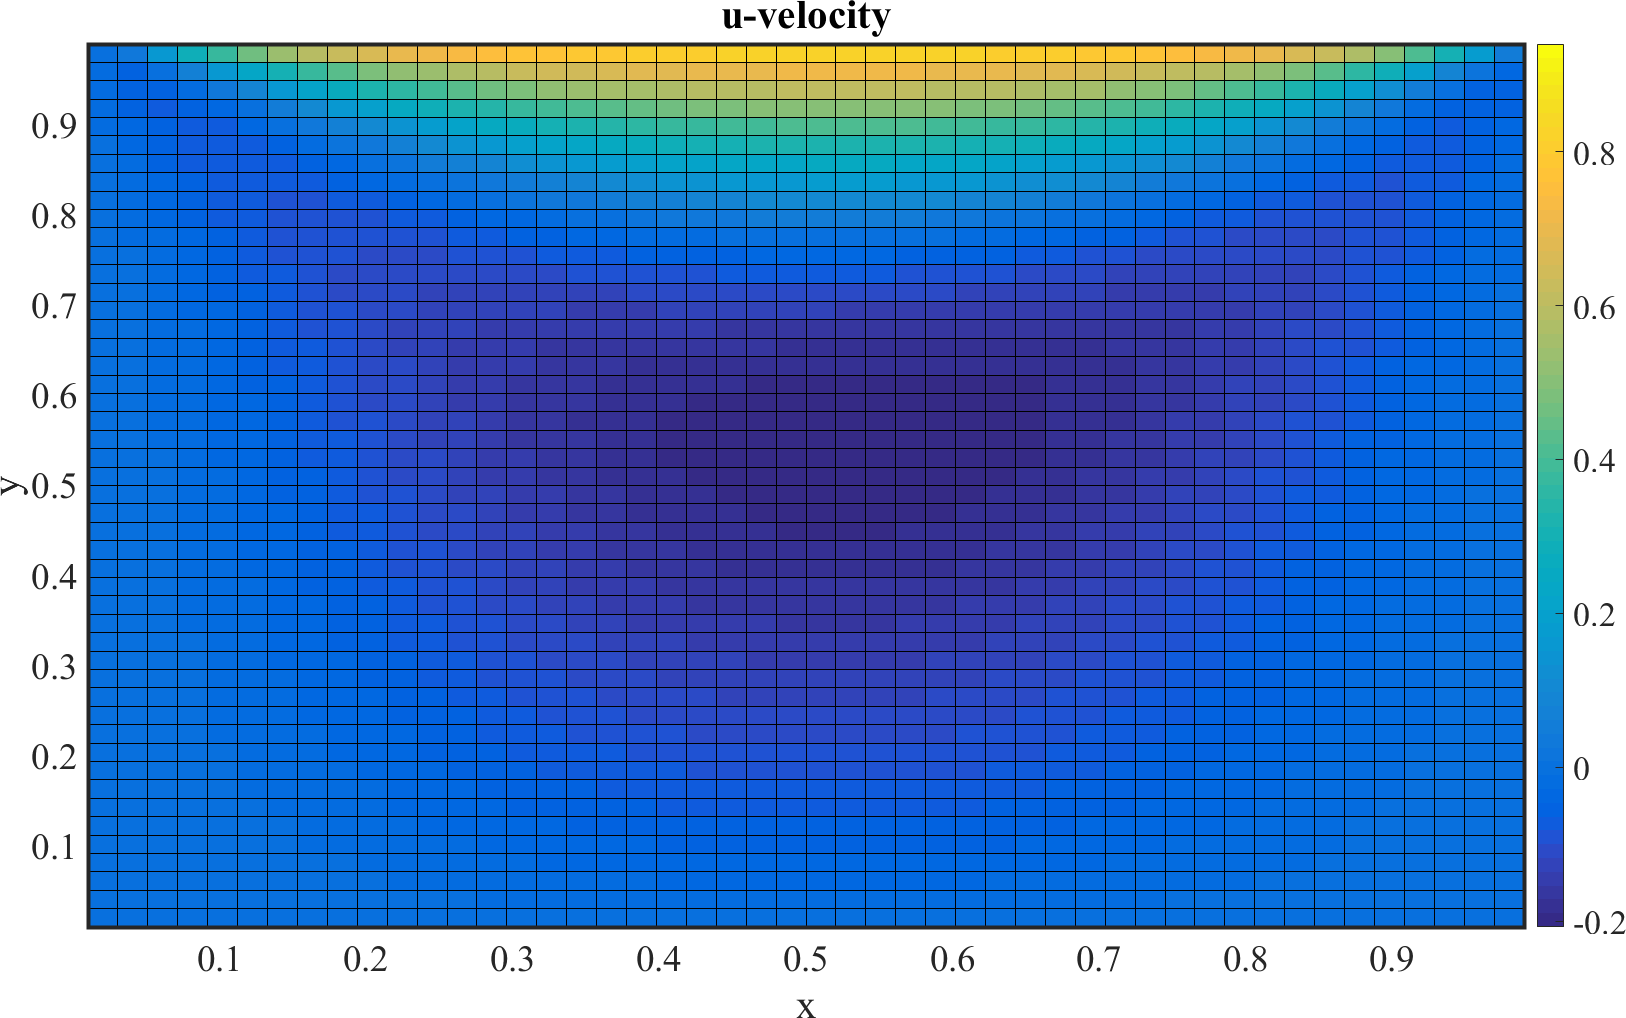
\includegraphics[clip,width=1\linewidth]{Re10u}

}%
\end{minipage}\hfill{}\centering%
\begin{minipage}[c]{0.49\textwidth}%
\subfloat[$v$\label{fig:Re1v}]{\centering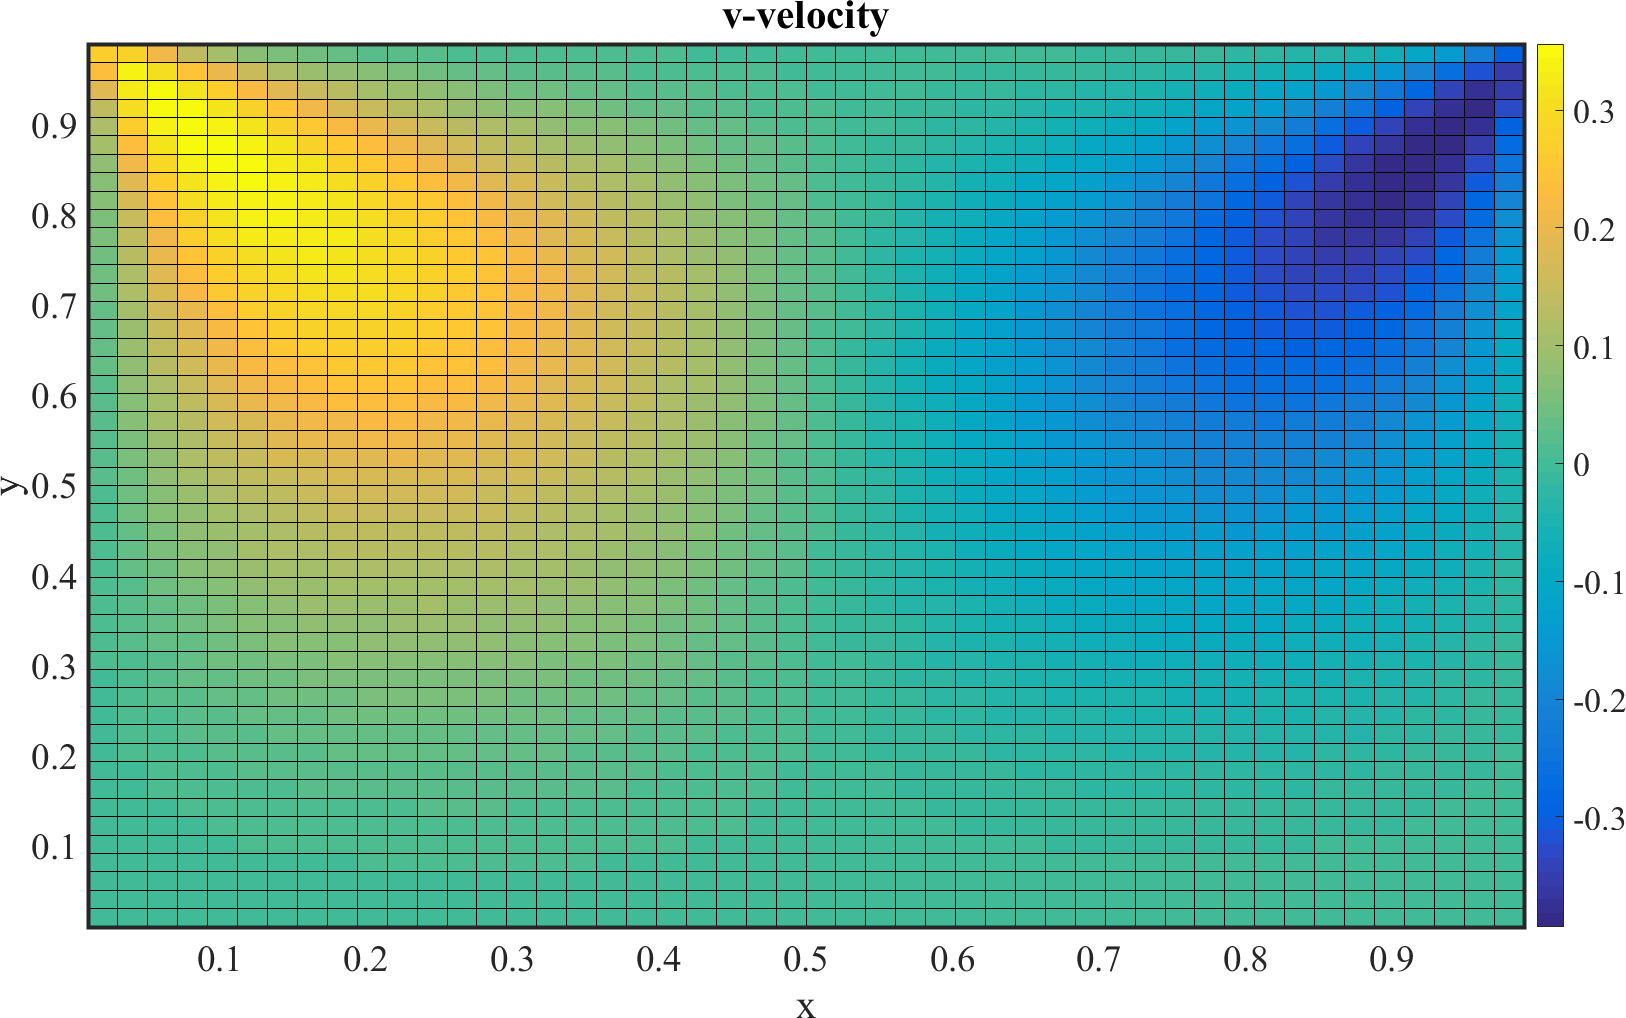
\includegraphics[clip,width=1\linewidth]{Re10v}

}%
\end{minipage}\medskip{}

\centering%
\begin{minipage}[c]{0.49\textwidth}%
\subfloat[Flow Speed \label{fig:Re1Speed}]{\centering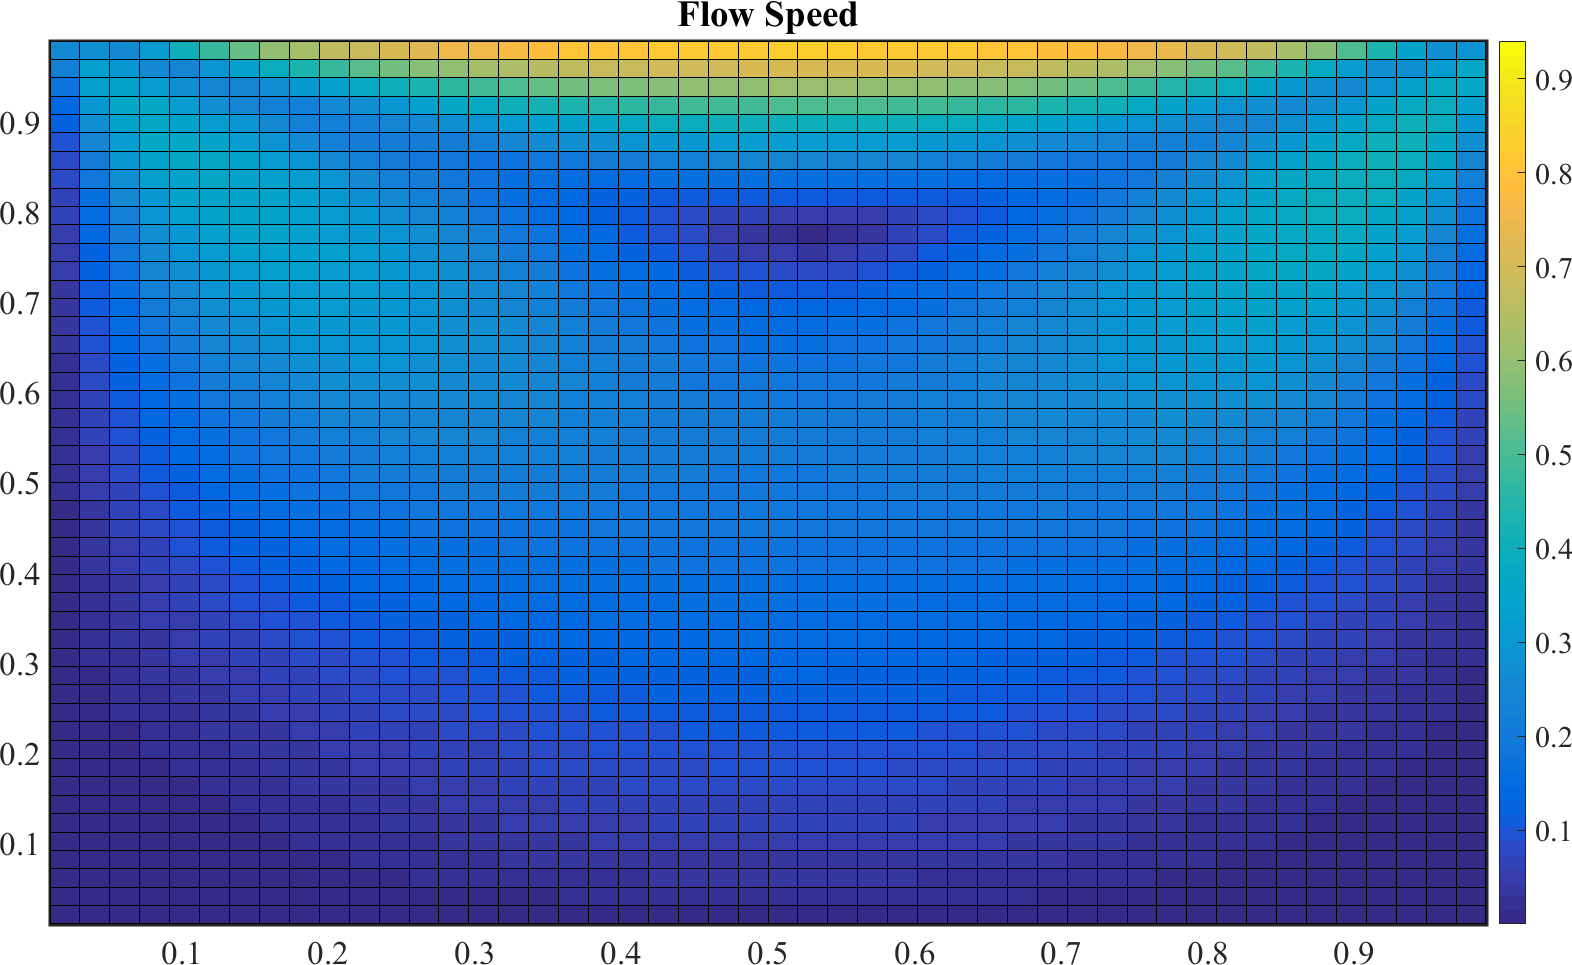
\includegraphics[clip,width=1\linewidth]{Re10Speed}

}%
\end{minipage}\hfill{}\centering%
\begin{minipage}[c]{0.49\textwidth}%
\subfloat[$\psi$\label{fig:Re1Stream}]{\centering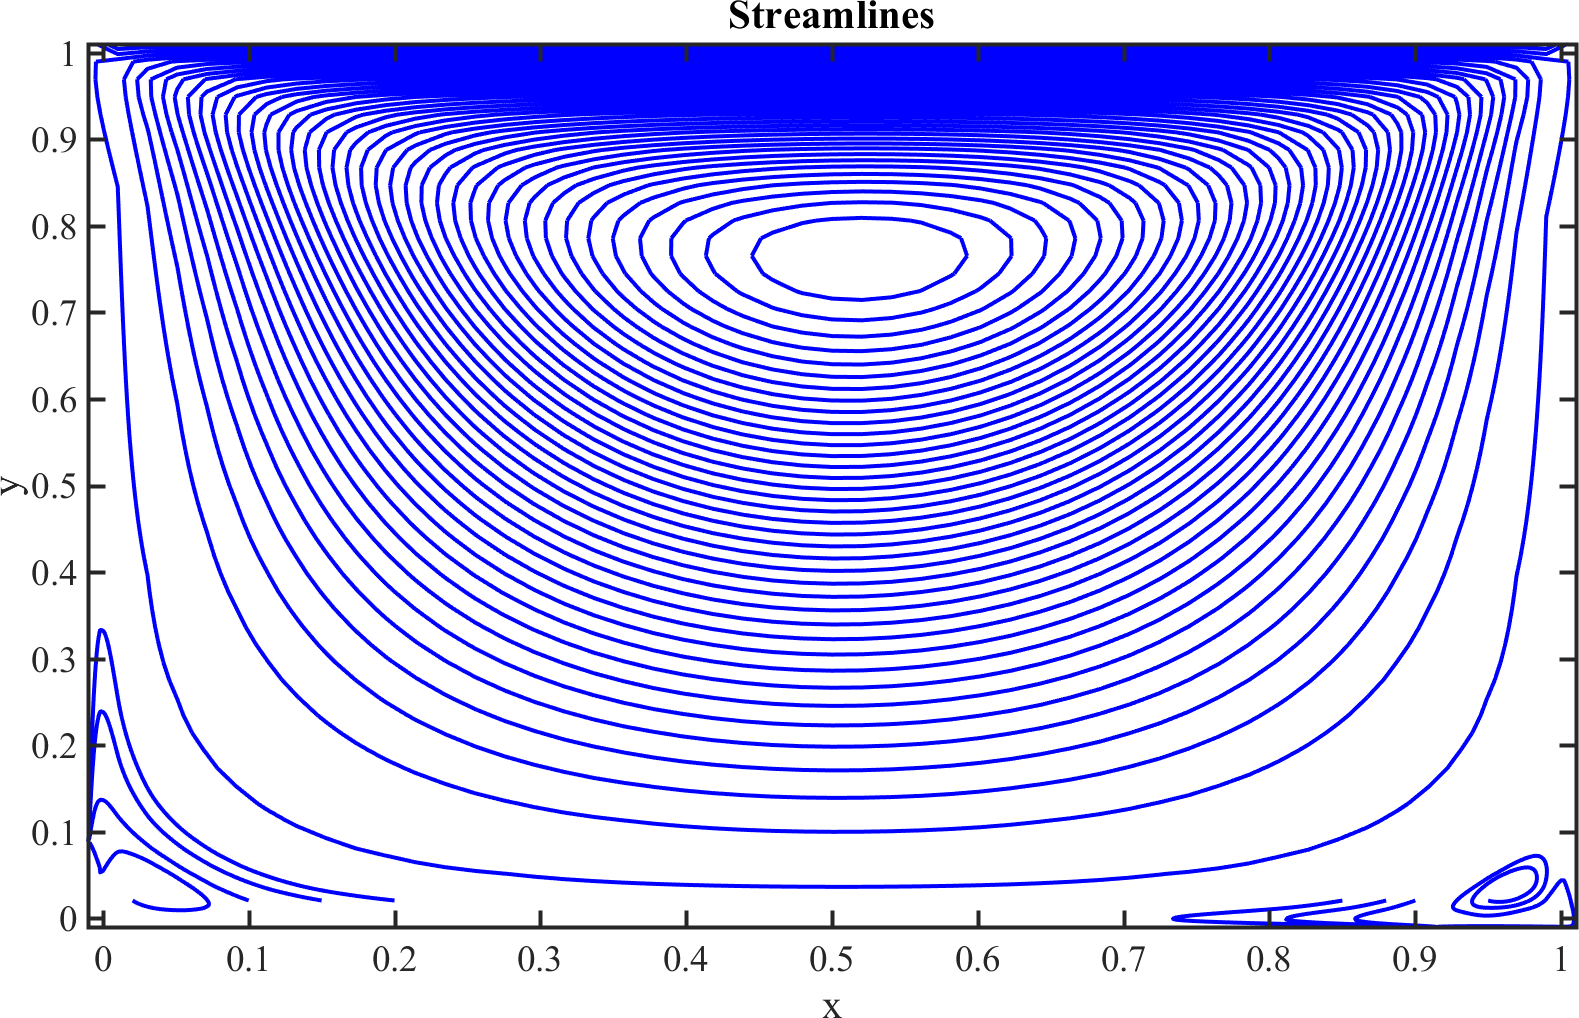
\includegraphics[clip,width=1\linewidth]{Re10Stream}

}%
\end{minipage}\caption{Results - Re 10\label{fig:Re1Results}}
\end{figure}

\begin{figure}[h]
\centering%
\begin{minipage}[c]{0.49\textwidth}%
\subfloat[$u$\label{fig:Re1u-1}]{\centering\includegraphics[clip,width=1\linewidth]{../../../Desktop/Project1/IC2}

}%
\end{minipage}\hfill{}\centering%
\begin{minipage}[c]{0.49\textwidth}%
\subfloat[$v$\label{fig:Re1v-1}]{\centering\includegraphics[clip,width=1\linewidth]{../../../Desktop/Project1/ContourCompare}

}%
\end{minipage}\medskip{}

\centering%
\begin{minipage}[c]{0.49\textwidth}%
\subfloat[Flow Speed \label{fig:Re1Speed-1}]{\centering\includegraphics[clip,width=1\linewidth]{../../../Desktop/Project1/IC2}

}%
\end{minipage}\hfill{}\centering%
\begin{minipage}[c]{0.49\textwidth}%
\subfloat[$\psi$\label{fig:Re1Stream-1}]{\centering\includegraphics[clip,width=1\linewidth]{../../../Desktop/Project1/ContourCompare}

}%
\end{minipage}\caption{Results - Re 100\label{fig:Re10Results}}
\end{figure}

\begin{figure}[h]
\centering%
\begin{minipage}[c]{0.49\textwidth}%
\subfloat[$u$\label{fig:Re1u-2}]{\centering\includegraphics[clip,width=1\linewidth]{../../../Desktop/Project1/IC2}

}%
\end{minipage}\hfill{}\centering%
\begin{minipage}[c]{0.49\textwidth}%
\subfloat[$v$\label{fig:Re1v-2}]{\centering\includegraphics[clip,width=1\linewidth]{../../../Desktop/Project1/ContourCompare}

}%
\end{minipage}\medskip{}

\centering%
\begin{minipage}[c]{0.49\textwidth}%
\subfloat[Flow Speed \label{fig:Re1Speed-2}]{\centering\includegraphics[clip,width=1\linewidth]{../../../Desktop/Project1/IC2}

}%
\end{minipage}\hfill{}\centering%
\begin{minipage}[c]{0.49\textwidth}%
\subfloat[$\psi$\label{fig:Re400Stream}]{\centering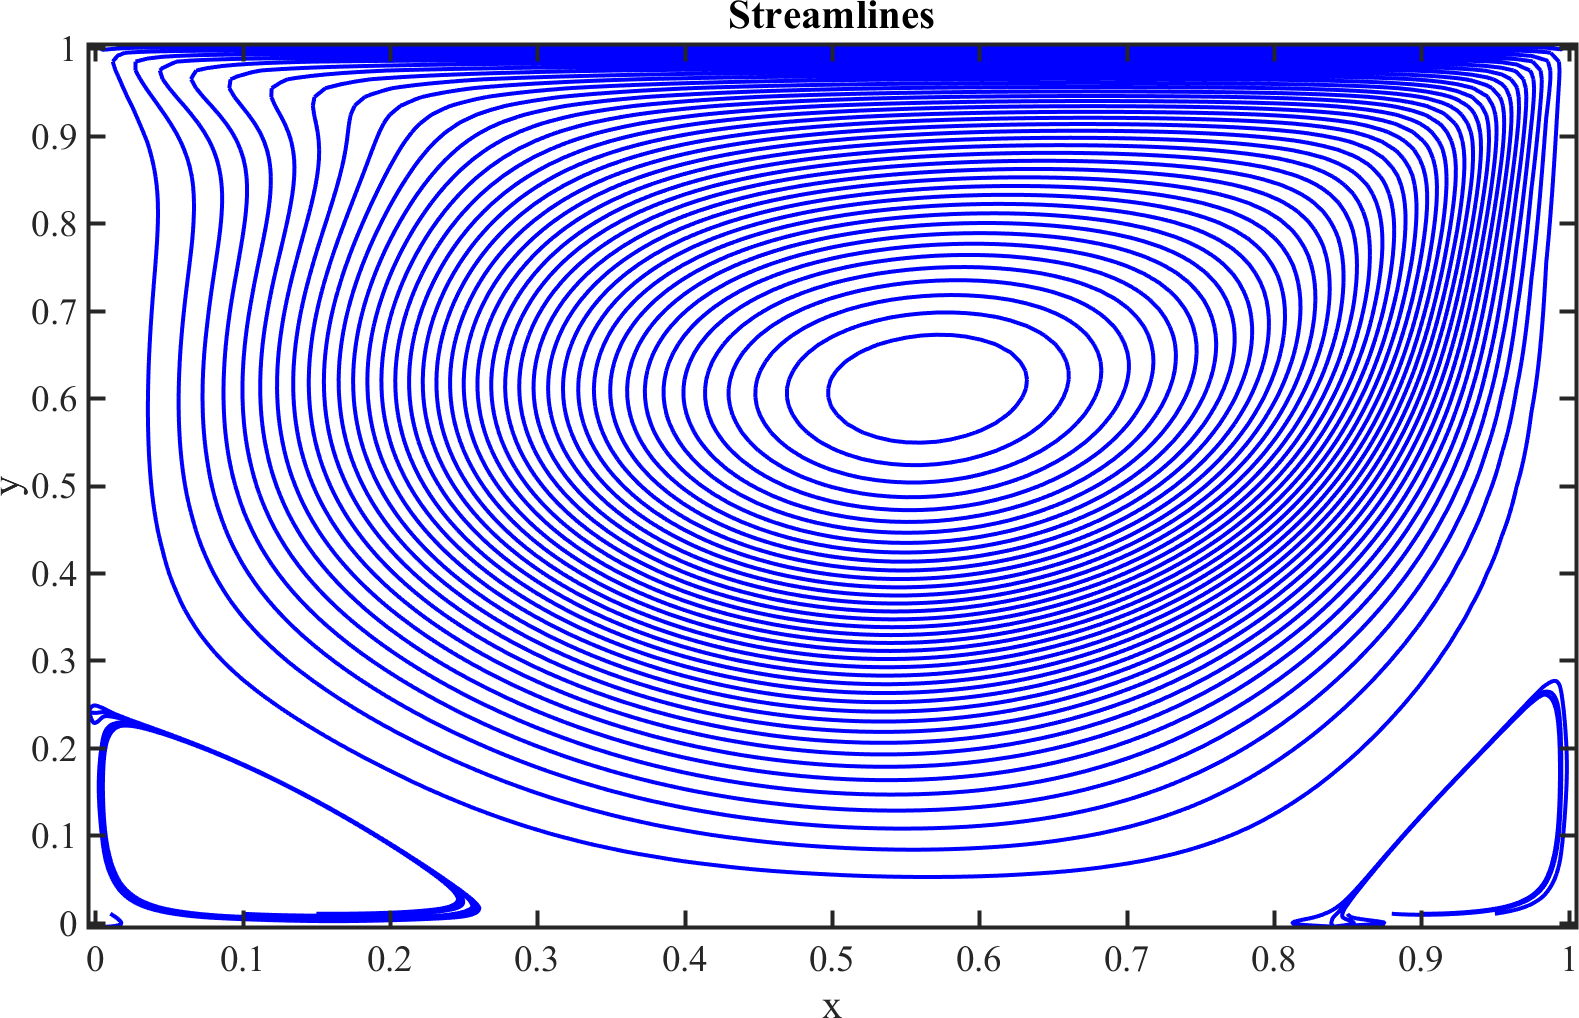
\includegraphics[clip,width=1\linewidth]{Re400Stream}

}%
\end{minipage}\caption{Results - Re 400\label{fig:Re400Results}}
\end{figure}

\begin{figure}[h]
\centering%
\begin{minipage}[c]{0.49\textwidth}%
\subfloat[$u$\label{fig:Re1u-3}]{\centering\includegraphics[clip,width=1\linewidth]{../../../Desktop/Project1/IC2}

}%
\end{minipage}\hfill{}\centering%
\begin{minipage}[c]{0.49\textwidth}%
\subfloat[$v$\label{fig:Re1v-3}]{\centering\includegraphics[clip,width=1\linewidth]{../../../Desktop/Project1/ContourCompare}

}%
\end{minipage}\medskip{}

\centering%
\begin{minipage}[c]{0.49\textwidth}%
\subfloat[Flow Speed \label{fig:Re1000Speed}]{\centering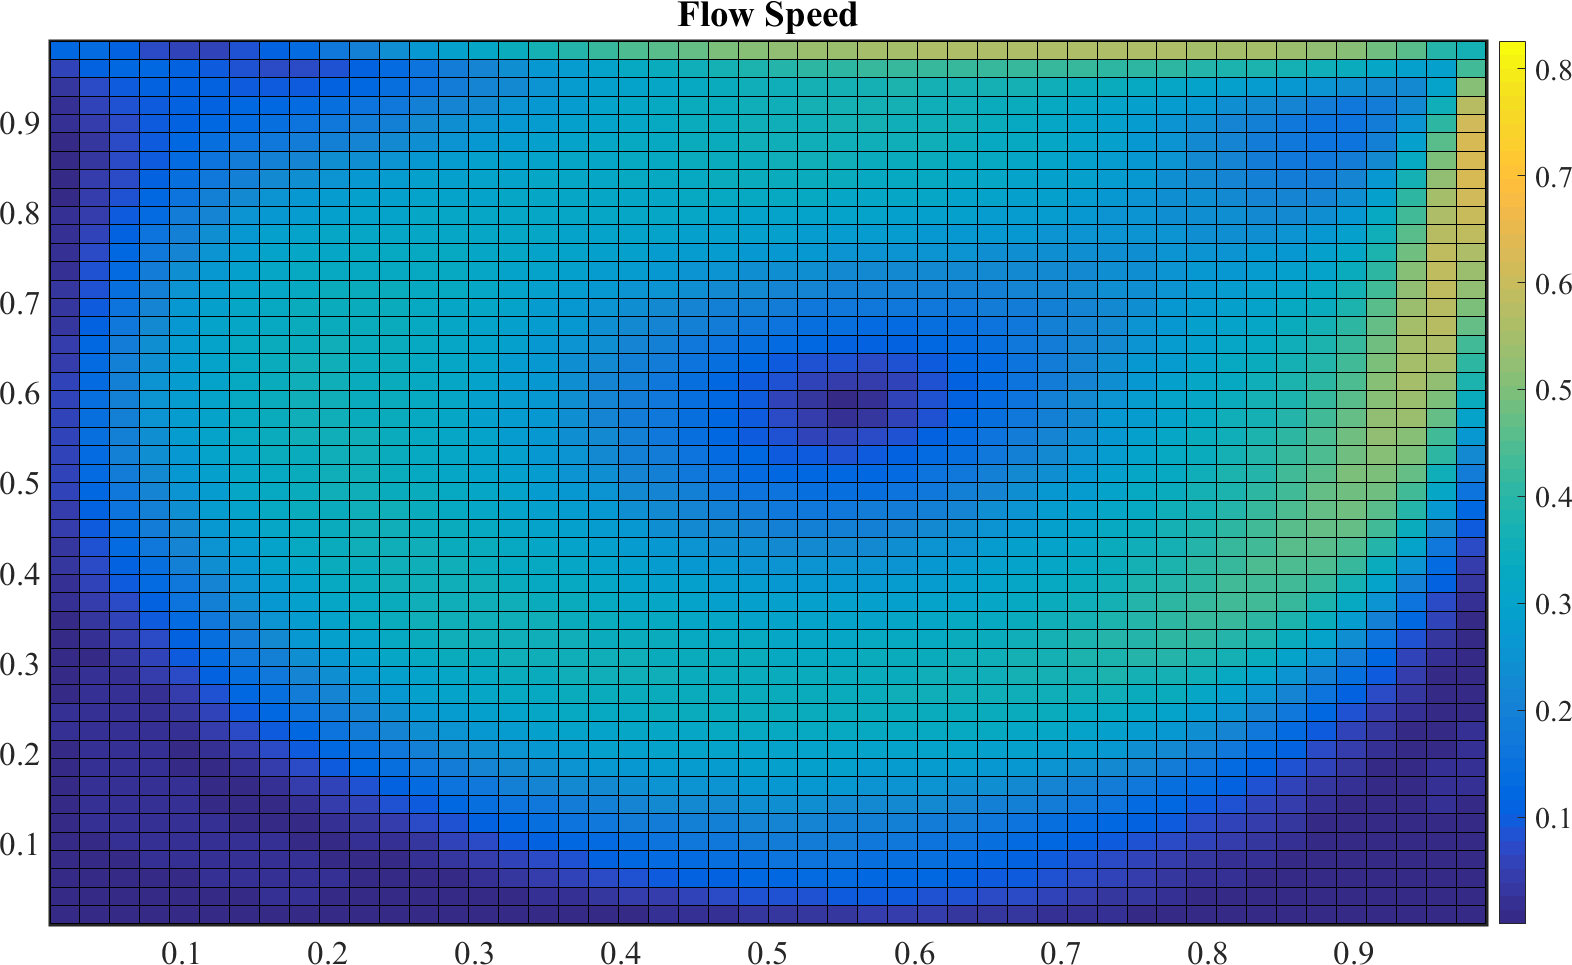
\includegraphics[clip,width=1\linewidth]{Re1000Speed}

}%
\end{minipage}\hfill{}\centering%
\begin{minipage}[c]{0.49\textwidth}%
\subfloat[$\psi$\label{fig:Re1000Stream}]{\centering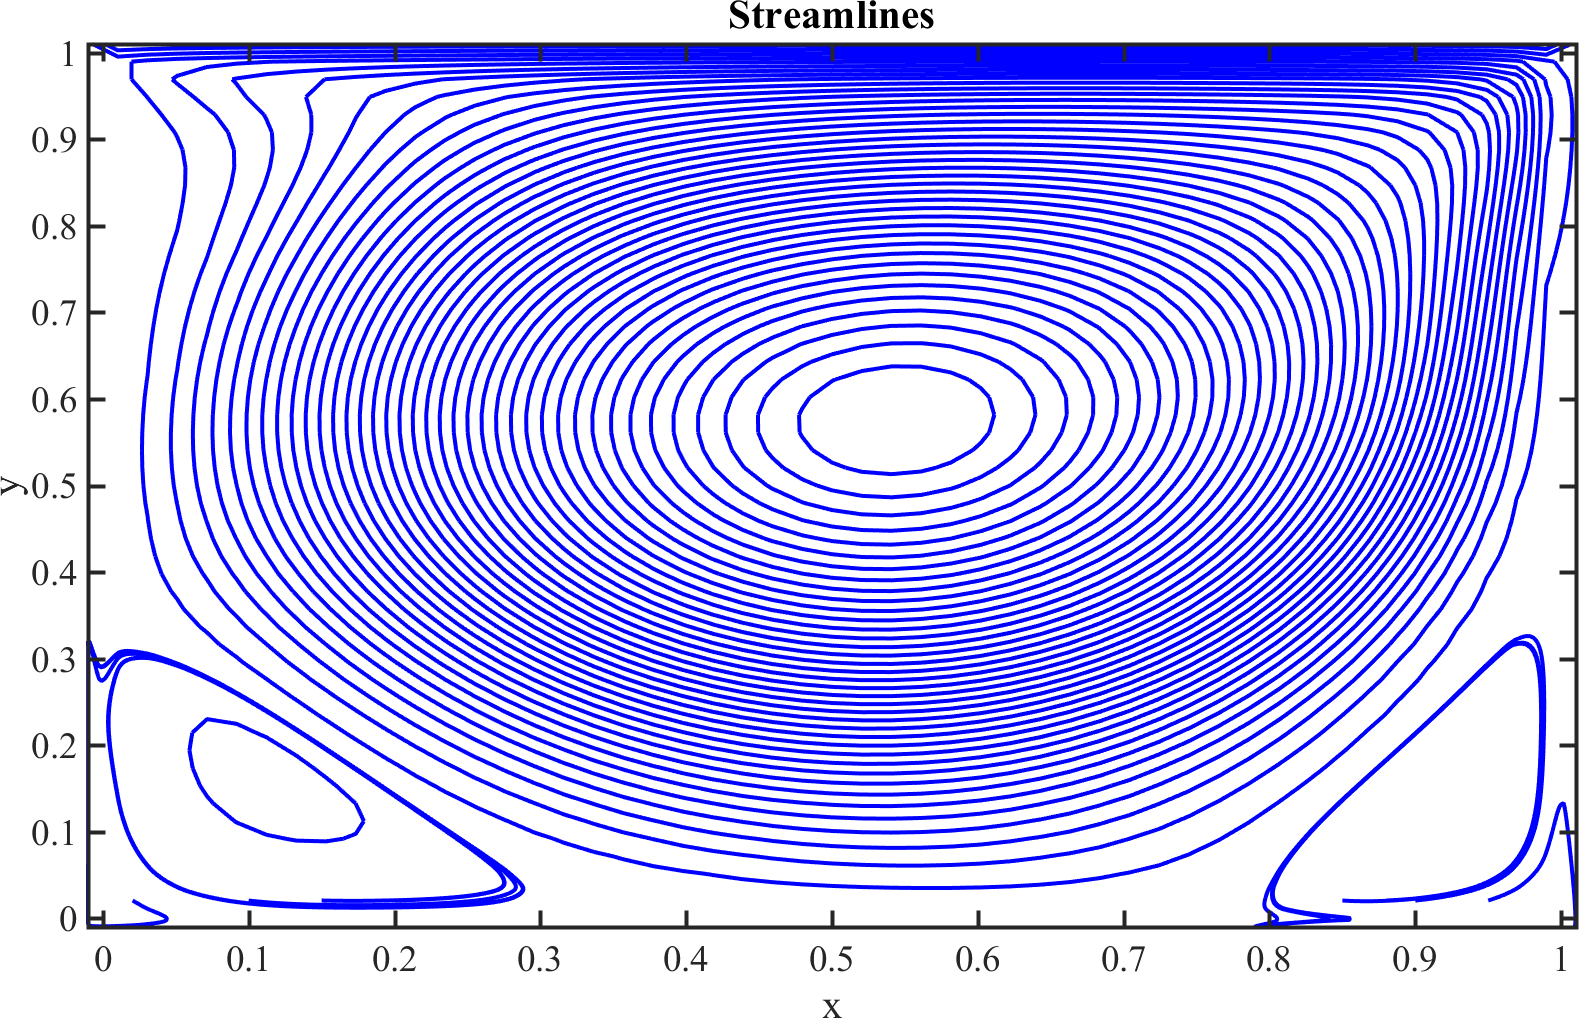
\includegraphics[clip,width=1\linewidth]{Re1000Stream}

}%
\end{minipage}\caption{Results - Re 1000\label{fig:Re1000Results}}
\end{figure}

While Figure \ref{fig:Re1v} does make it clear that \textit{some
}change in the results did indeed occur due to the modified corner
boundary, in order to both better understand the effect of geometry
on the flow patterns within the box and provided validation for the
geometry adjustment method used, the domain of analysis was further
restricted by removing all nodes beyond the boundary identified in
Figure \ref{fig:Diagram} as the ``Modified Wall''. Unsurprisingly,
moving the wall this far into the domain proved to have a much larger
effect.

\begin{figure}[h]
\centering%
\begin{minipage}[c]{0.49\textwidth}%
\subfloat[Re 400\label{fig:CenterlineCompare400}]{\centering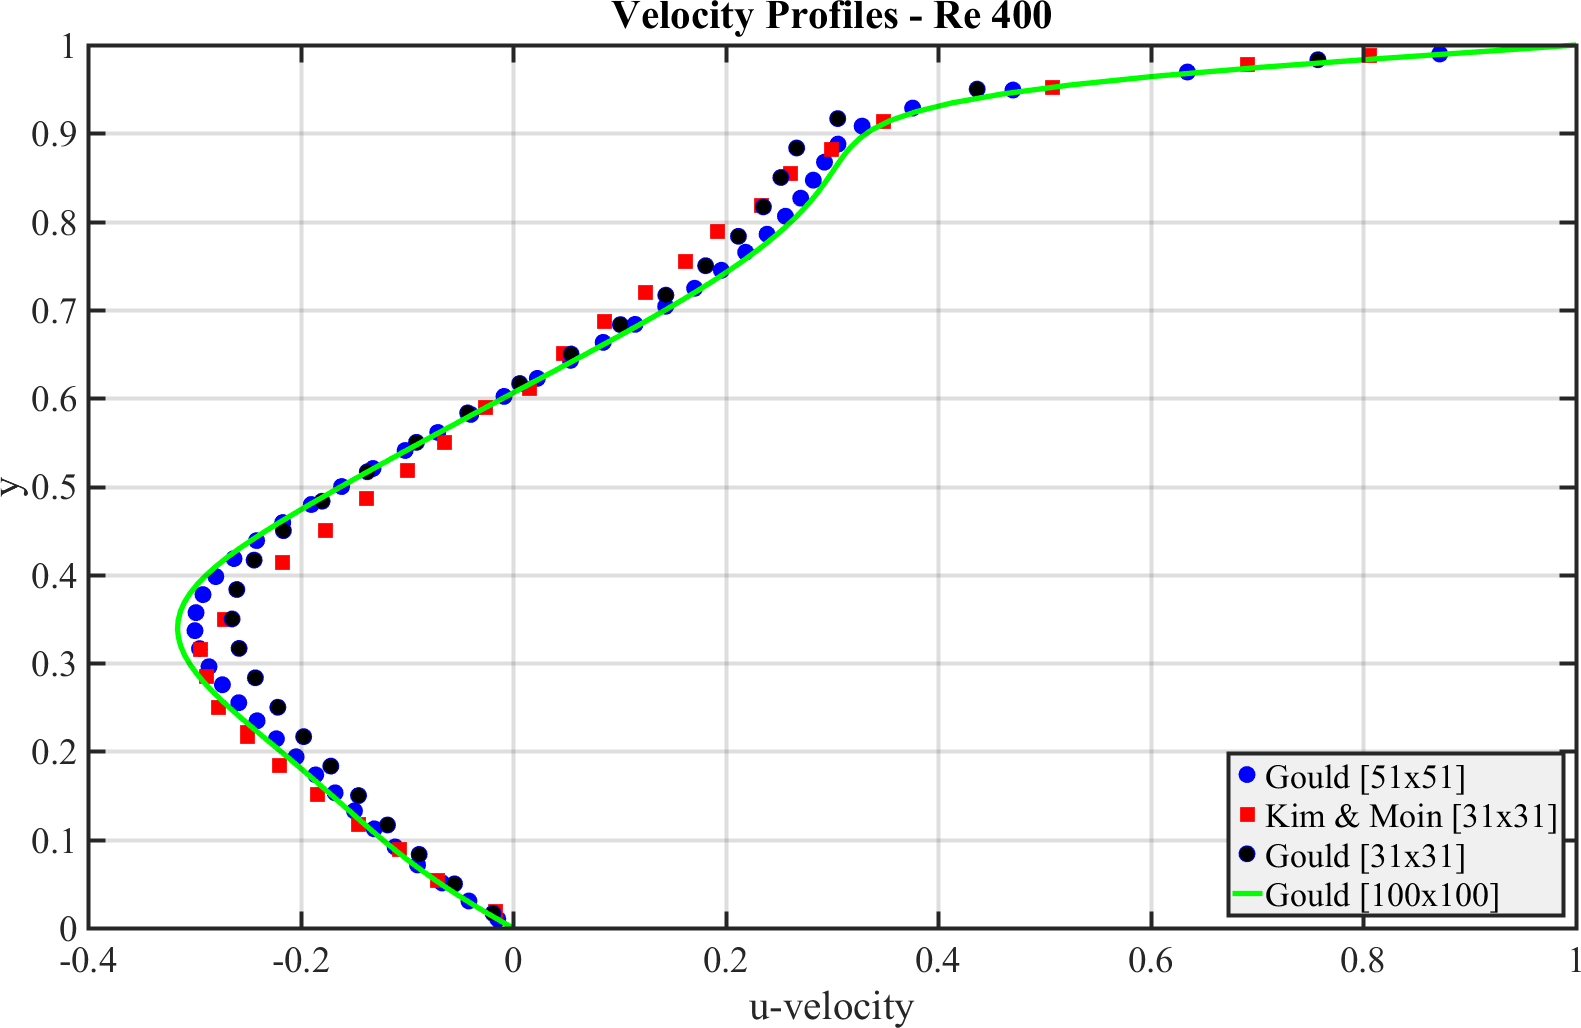
\includegraphics[clip,width=1\linewidth]{Re400profiles}

}%
\end{minipage}\hfill{}\centering%
\begin{minipage}[c]{0.49\textwidth}%
\subfloat[Re400\label{fig:CenterlineCompare1000}]{\centering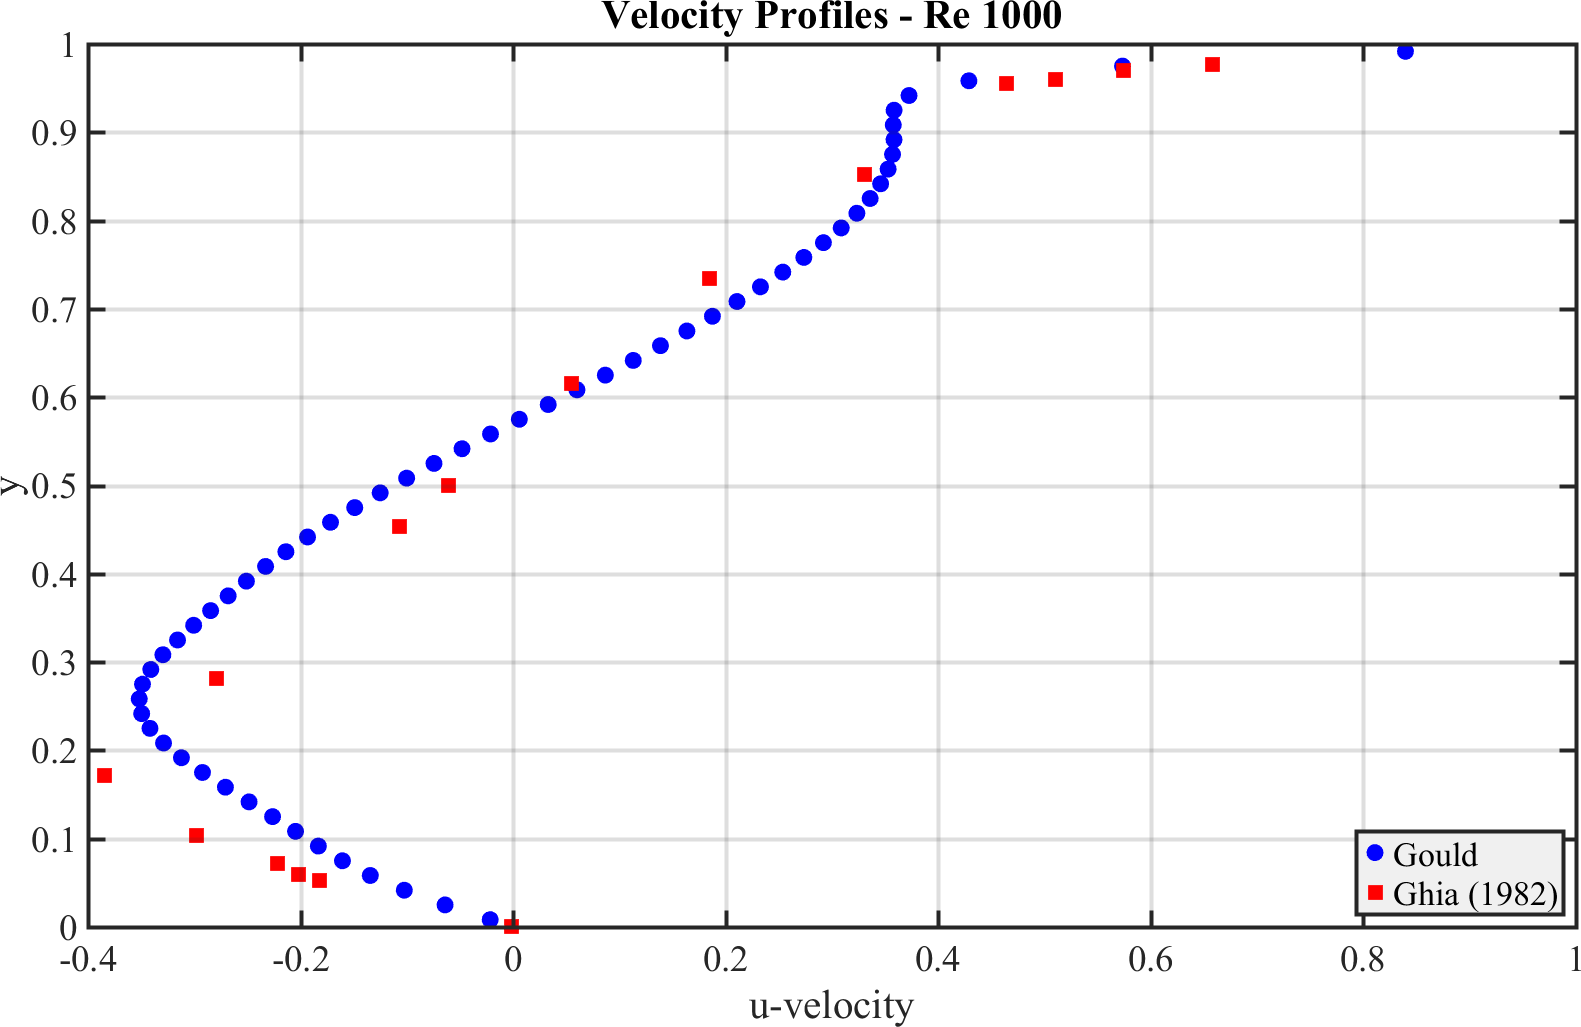
\includegraphics[clip,width=1\linewidth]{CenterlineVelocityRe1000}

}%
\end{minipage}\caption{Comparison of calculated $u$ velocity along cavity centerline \label{fig:CenterlineCompare}}
\end{figure}

Finally, to further disturb the flow, a partial barrier was added
in the region between the inlet and outlet by assigning a line of
nodes at x=3m to be equal 0. This assignment created a new wall attached
to the wall between points A and C. This is seen in Figure \ref{fig:ICbarrier}.
Unsurprisingly, the addition of the barrier worked in conjunction
with the extended wall and resulted in a highly disturbed flow path.
A contour and pseudocolor plot depicting this is presented in Figure
\ref{fig:imageContour}. The code calculating this effect is provided
in Appendix \ref{subsec:Problem-2-w/}.

\begin{figure}[h]
\centering%
\begin{minipage}[c]{0.49\textwidth}%
\subfloat[Initial conditions for simulation with barrier\label{fig:ICbarrier}]{\centering\includegraphics[clip,width=1\linewidth]{../../../Desktop/Project1/ICBarrier}

}%
\end{minipage}\hfill{}\centering%
\begin{minipage}[c]{0.49\textwidth}%
\subfloat[Effect of barrier on solution \label{fig:imageContour}]{\centering\includegraphics[clip,width=1\linewidth]{../../../Desktop/Project1/SolutionBarrierContour}

}%
\end{minipage}\caption{Modified geometry - shape and barrier \label{fig:Barrier}}
\end{figure}


\section{Conclusion}

Despite the limited resolution, the methods employed in solving the
Laplace equation for the stream function within the domain of interest
proved to be very effective. Regarding the different solution methods,
it was found that when using Matlab, the ability to vectorize an equation
is of significant importance. This is admittedly a significant drawback
if one is going to be using the language for iterative solutions to
finite difference equations. Unfortunately, it was also discovered
by the author that all other coding options are horrible and evil.
Thus, in the future, this author would recommend that FDE equations
can be best solved by either using working in Matlab and using Matlab's
built in, vectorized functions as much as possible, or simply buying
some computer science grad student a 6 pack of beer to program the
solution code for you in a awful, but fast language such as C or Fortran.
\end{document}
